

\chapter{Flight simulation}
\label{chap-simulation}

In this chapter the actual flight simulation is analyzed.  First in
Section~\ref{sec-atmospheric-properties} methods for simulating
atmospheric conditions and wind are presented.  Then in
Section~\ref{sec-flight-modeling} the actual simulation procedure is
developed.



\section{Atmospheric properties}
\label{sec-atmospheric-properties}

In order to calculate the aerodynamic forces acting on the rocket it
is necessary to know the prevailing atmospheric conditions.  Since the
atmosphere is not constant with altitude, a model must be developed to
account for the changes.  Wind also plays an important role in the
flight of a rocket, and therefore it is important to have a realistic
wind model in use during the simulation.


\subsection{Atmospheric model}

The atmospheric model is responsible to estimating the atmospheric
conditions at varying altitudes.  The properties that are of most
interest are the density of air $\rho$ (which is a scaling parameter
to the aerodynamic coefficients via the dynamic pressure
$\frac{1}{2}\rho v^2$) and the speed of sound $c$ (which affects the
Mach number of the rocket, which in turn affects its aerodynamic
properties).  These may in turn be calculated from the air pressure
$p$ and temperature $T$.

Several models exist that define standard atmospheric conditions as a
function of altitude, including the Internaltional Standard
Atmosphere (ISA)~\cite{international-standard-atmosphere} and the
U.S. Standard Atmosphere~\cite{US-standard-atmosphere}.  These two
models yield identical temperature and pressure profiles for altitudes
up to 32~km.

The models are based on the assumption that air follows the ideal gas
law
%
\begin{equation}
\rho = \frac{Mp}{RT}
\end{equation}
%
where $M$ is the molecular mass of air and $R$ is the ideal gas
constant.  From the equilibrium of hydrostatic forces the differential
equation for pressure as a function of altitude $z$ can be found as
%
\begin{equation}
\dif p = -g_0 \rho \dif z = -g_0 \frac{Mp}{RT} \dif z
\label{eq-pressure-altitude}
\end{equation}
%
where $g_0$ is the gravitational acceleration.  If the temperature of
air were to be assumed to be constant, this would yield an exponential
diminishing of air pressure.

The ISA and U.S. Standard Atmospheres further specity a standard
temperature and pressure at sea level and a temperature profile for
the atmosphere.  The temperature profile is given as eight
temperatures for different altitudes, which are then linearly
interpolated.  The temperature profile and base pressures for the ISA
model are presented in Table~\ref{table-ISA-model}.  These values
along with equation~(\ref{eq-pressure-altitude}) define the
temperature/pressure profile as a function of altitude.

\begin{table}
\caption{Layers defined in the International Standard
  Atmosphere~\cite{wiki-ISA-layers}}
\label{table-ISA-model}
\begin{center}
\begin{tabular}{ccccl}
\hline
Layer & Altitude$^\dagger$ & Temperature & Lapse rate &
                                                \multicolumn{1}{c}{Pressure} \\
      &  m       &  $^\circ$C  & $^\circ$C/km & \multicolumn{1}{c}{Pa} \\
\hline
0     & 0        & $+15.0$     & $-6.5$       & 101\s325 \\
1     & 11\s000  & $-56.5$     & $+0.0$       & \num22\s632 \\
2     & 20\s000  & $-56.5$     & $+1.0$       & \num\num5\s474.9 \\
3     & 32\s000  & $-44.5$     & $+2.8$       & \num\num\num\s868.02 \\
4     & 47\s000  & \num$-2.5$  & $+0.0$       & \num\num\num\s110.91 \\
5     & 51\s000  & \num$-2.5$  & $-2.8$       & \num\num\num\s\num66.939 \\
6     & 71\s000  & $-58.5$     & $-2.0$       & \num\num\num\s\num\num3.9564 \\
7     & 84\s852  & $-86.2$     &              & \num\num\num\s\num\num0.3734 \\
\hline
\end{tabular}
\end{center}
\vspace{-3mm}
{\footnotesize $^\dagger$ Altitude is the geopotential height which
  does not account for the diminution of gravity at high altitudes.}
\vspace{3mm}
\end{table}

These models are totally static and do not take into account any local
flight conditions.  Many rocketeers may be interested in flight
differences during summer and winter and what kind of effect air pressure
has on the flight.  These are also parameters that can easily be
measured on site when launching rockets.  On the other hand, it is
generally hard to know a specific temperature profile for a specific
day.  Therefore the atmospheric model was extended to allow the user
to specify the base conditions either at mean sea level or at the
altitude of the launch site.  These values are simply assigned to the
first layer of the atmospheric model.  Most model rockets do not
exceed altitudes of a few kilometers, and therefore the flight
conditions at the launch site will dominate the flight.

One parameter that also has an effect on air density and the speed of
sound is humidity.  The standard models do not include any definition
of humidity as a function of altitude.  Furthermore, the effect of
humidity on air density and the speed of sound is marginal.  The
difference in air density and the speed of sound between completely dry
air and saturated air at standard conditions are both less than 1\%.
Therefore the effect of humidity has been ignored.




\subsection{Wind modeling}

Wind plays a critical role in the flight of model rockets.  As has
been seen, large angles of attack may cause rockets to lose a
significant amount of stability and even go unstable.  Over-stable
rockets may weathercock and turn into the wind.  In a perfectly static
atmosphere a rocket would, in principle, fly its entire flight
directly upwards at zero angle of attack.  Therefore, the effect of
wind must be taken into account in a full rocket simulation.

Most model rocketeers, however, do not have access to a full wind
profile of the area they are launching in.  Different layers of air
may have different wind velocities and directions.  Modeling such
complex patterns is beyond the scope of this project. Therefore, the
goal is to produce a realistic wind model that can be specified with
only a few parameters understandable to the user and that covers
altitudes of most rocket flights.  Extensions to allow for multiple
air layers may be added in the future.

In addition to a constant average velocity, wind always has some
degree of turbulence in it.  The effect of turbulence can be modeled
by summing the steady flow of air and a random, zero-mean turbulence
velocity.  Two central aspects of the turbulence velocity are the
amplitude of the variation and the frequencies at which they occur.
Therefore a reasonable turbulence model is achieved by a random
process that produces a sequence with a similar distribution and
frequency spectrum as that of real wind.

Several models of the spectrum of wind turbulence at specific
altitudes exist.  Two commonly used such spectra are the {\it Kaimal}
and {\it von K�rm�n} wind turbulence
spectra~\cite[p.~23]{wind-energy-handbook}:
%
\begin{eqnarray}
\mbox{Kaimal:} & & \frac{S_u(f)}{\sigma_u^2} =
    \frac{4 L_{1u} / U}{(1 + 6fL_{1u}/U)^{5/3}} \label{eq-kaimal-wind} \\
%
\mbox{von K�rm�n:} & & \frac{S_u(f)}{\sigma_u^2} =
    \frac{4 L_{2u} / U}{(1 + 70.8(fL_{2u}/U)^2)^{5/6}} \label{eq-karman-wind}
\end{eqnarray}

Here $S_u(f)$ is the spectral density function of the turbulence
velocity and $f$ the turbulence frequency, $\sigma_u$ the standard
deviation of the turbulence velocity, $L_{1u}$ and $L_{2u}$ length
parameters and $U$ the average wind speed.

Both models approach the asymptotic limit 
$S_u(f)/\sigma_u^2 \sim f^{-5/3}$ quite fast.  Above frequencies of
0.5~Hz the difference between equation~(\ref{eq-kaimal-wind}) and the
same equation without the term 1 in the denominator is less than 4\%.
Since the time scale of a model rocket's flight is quite short, the
effect of extremely low frequencies can be ignored.  Therefore
turbulence may reasonably well be modelled by utilizing 
{\it pink noise} that has a spectrum of $1/f^\alpha$ with $\alpha=5/3$.
True pink noise has the additional useful property of being
scale-invariant.  This means that a stream of pink noise samples may
be generated and assumed to be at any sampling rate while maintaining
their spectral properties.

Discerete samples of pink noise with spectrum $1/f^\alpha$ can be
generated by applying a suitable digital filter to {\it white noise},
which is simply uncorrelated pseudorandom numbers.  One such filter is
the infinite impulse response (IIR) filter presented by
Kasdin~\cite{pink-filter}:
%
\begin{equation}
x_n = w_n - a_1 x_{n-1} - a_2 x_{n-2} - a_3 x_{n-3} - \ldots
\label{eq-pink-generator}
\end{equation}
%
where $x_i$ are the generated samples, $w_n$ is a generated white
random number and the coefficients are computed using
%
\begin{equation}
\begin{array}{rl}
a_0 & = 1 \\
a_k & = \del{k-1-\frac{\alpha}{2}} \frac{a_{k-1}}{k}.
\end{array}
\label{eq-pink-coefficients}
\end{equation}
%
The infinite sum may be truncated with a suitable number of terms.
In the context of IIR filters these terms are calles {\it poles}.
Experimentation showed that already 1--3 poles provides a reasonably
accurate frequency spectrum in the high frequency range.

One problem in using pink noise as a turbulence velocity
model is that the power spectrum of pure pink noise goes to
infinity at very low frequencies.  This means that a long sequence
of random values may deviate significantly from zero.  However, when
using the truncated IIR filter of equation~(\ref{eq-pink-generator}),
the spectrum density becomes constant below a certain limiting
frequency, dependent on the number of poles used.  By adjusting the
number of poles used, the limiting frequency can be adjusted to a value
suitable for model rocket flight.  Specifically, the number of poles
must be selected such that the limiting frequency is suitable at the
chosen sampling rate.  

It is also desirable that the simulation resolution does not affect
the wind conditions.  For example, a simulation with a time step of
10~ms should experience the same wind conditions as a simulation with
a time step of 5~ms.  This is achieved by selecting a constant
turbulence generation frequency and interpolating between the
generated points when necessary.  The fixed frequency was chosen at
20~Hz, which can still simulate fluctuations at a time scale of 0.1
seconds.

\begin{figure}[p]
\centering
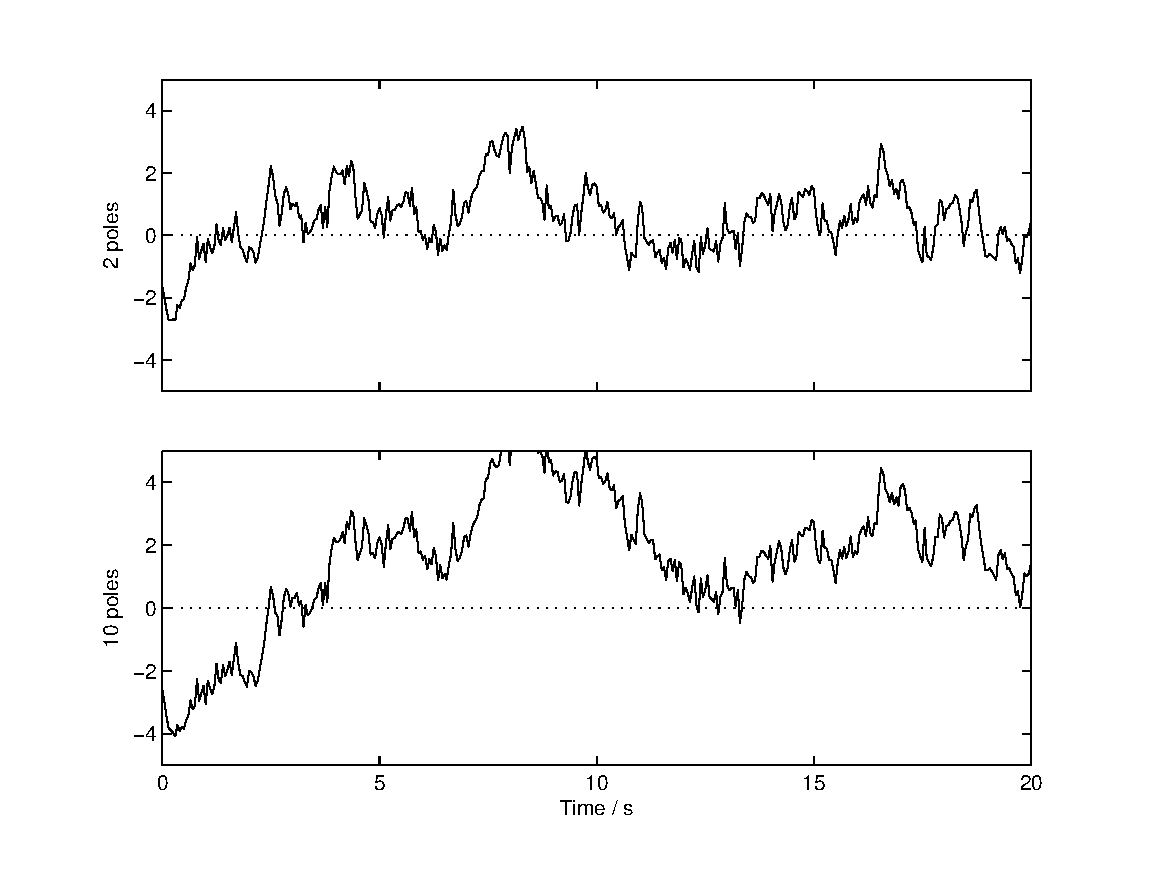
\epsfig{file=figures/wind/pinktime, width=105mm}
\caption{The effect of the number of IIR filter poles on two 20 second
  samples of generated turbulence, normalized so that the two-pole
  sequence has standard deviation one.}
\label{fig-pink-poles}
\end{figure}

\begin{figure}[p]
\centering
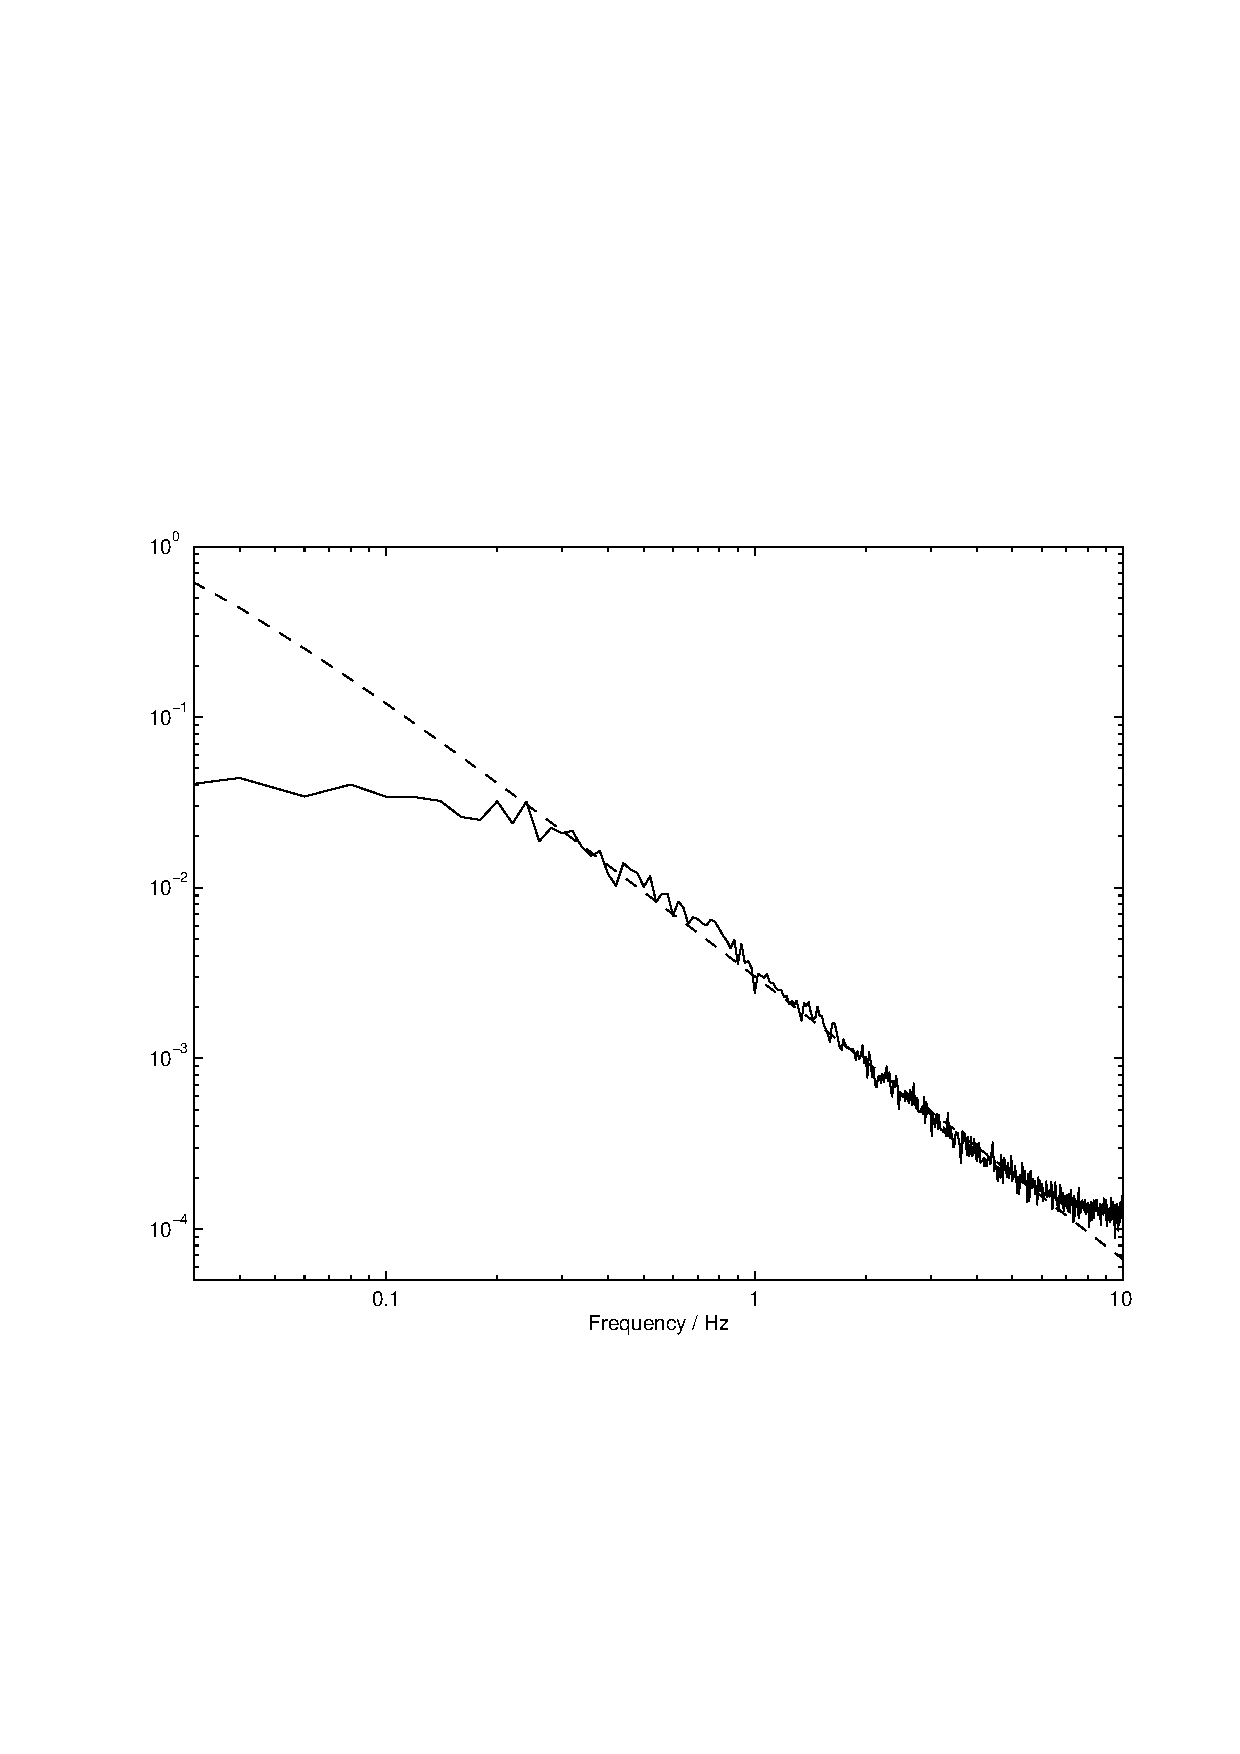
\epsfig{file=figures/wind/pinkfreq, width=95mm}
\caption{The average power spectrum of 100 turbulence
  simulations using a two-pole IIR filter (solid) and the Kaimal
  turbulence spectrum (dashed); vertical axis arbitrary.}
\label{fig-pink-spectrum}
\end{figure}



The effect of the number of poles is depicted in
Figure~\ref{fig-pink-poles}, where two pink noise sequences were
generated from the same random number source with two-pole and
ten-pole IIR filters.  A small number of poles generates values strongly
centered on zero, while a larger number of poles introduces more low
frequency variability.  Since the free-flight time of a typical model
rocket is of the order of 5--30 seconds, it is desireable that the
maximum gust length during the flight is substantially shorter than
this.  Therefore the pink noise generator used by the wind model was
chosen to contain only two poles, which has a limiting frequency of
approximately 0.3~Hz when sampled at 20~Hz.  This means that gusts of
wind longer than 3--5 seconds will be rare in the simulted turbulence,
which is a suitable gust length for modeling typical model rocket
flight. Figure~\ref{fig-pink-spectrum} depicts the resulting pink
noise spectrum of the two-pole IIR filter and the Kaimal spectrum of
equation~(\ref{eq-kaimal-wind}) scaled to match each other.


%, which causes frequency
%components below approximately 0.3~Hz to be subdued.  Therefore, gusts
%of wind longer than 3--5 seconds will be rare in the simulated wind, a
%suitable time scale for the flight of a model rocket.
%Figure~\ref{fig-turbulence}(a) shows a 20 second sample of the
%generated turbulence, normalized to have a standard deviation of one.
%Figure~\ref{fig-turbulence}(b) depicts the actual frequency spectrum
%of the generated turbulence and the Kaimal spectrum of
%equation~(\ref{eq-kaimal-wind}) scaled to match each other.



To simplify the model, the average wind speed is assumed to be
constant with altitude and in a constant direction.  This allows
specifying the model parameters using just the average wind speed and
its standard deviation.  An alternative parameter for specifying the
turbulence amplitude is the {\it turbulence intensity}, which is the
percentage that the standard deviation is of the average wind
velocity,
%
\begin{equation}
I_u = \frac{\sigma_u}{U}.
\end{equation}
%
Wind farm load design standards typically specify turbulence
intensities around 10\ldots20\%~\cite[p.~22]{wind-energy-handbook}.
It is assumed that these intensities are at the top of the range of
conditions in which model rockets are typically flown.

Overall, the process to generate the wind velocity as a function of
time from the average wind velocity $U$ and standard deviation
$\sigma_u$ can be summarized in the following steps:
%
\begin{enumerate}
%\item[Input:]  Average wind velocity $U$ and standard deviation
%  $\sigma_u$.
%
\item Generate a pink noise sample $x_n$ from a Gaussian white noise
  sample $w_n$ using equations~(\ref{eq-pink-generator}) and
  (\ref{eq-pink-coefficients}) with two memory terms included.

\item Scale the sample to a standard deviation one.  This is performed
  by dividing the value by a previously calculated standard deviation
  of a long, unscaled pink noise sequence (2.252 for the two-pole IIR
  filter).

\item The wind velocity at time $n\cdot\Delta t$ ($\Delta t = 0.05\rm~s$)
  is $U_n = U + \sigma_u x_n$.  Velocities in between are interpolated.
\end{enumerate}




\section{Modeling rocket flight}
\label{sec-flight-modeling}


Modeling of rocket flight is based on Newton's laws.  The basic forces
acting upon a rocket are gravity, thrust from the motors and
aerodynamic forces and moments.  These forces and moments are
calculated and integrated numerically to yield a simulation over a
full flight.

Since most model rockets fly at a maximum a few kilometers high, the
curvature of the Earth is not taken into account.  Assuming a flat
Earth allows us to use simple Cartesian coordinates to represent the
position and altitude of the rocket.  As a consequence, the coriolis
effect when flying long distances north or south is not simulated
either.



\subsection{Coordinates and orientation}

During a rocket's flight many quantities, such as the aerodynamical
forces and thrust from the motors, are relative to the rocket itself,
while others, such as the position and gravitational force, are more
naturally described relative to the launch site.  Therefore two sets
of coordinates are defined, the {\it rocket coordinates}, which are
the same as used in Chapter~\ref{chap-aerodynamics}, and 
{\it world coordinates}, which is a fixed coordinate system with the
origin at the position of launch.

The position and velocity of a rocket are most naturally maintained as
Cartesian world coordinates.  Following normal convensions, the
$xy$-plane is selected to be parallel to the ground and the $z$-axis
is chosen to point upwards.  In flight dynamics of aircraft the
$z$-axis often points towards the earth, but in the case of rockets it
is natural to have the rocket's altitude as the $z$-coordinate.

Since the wind is assumed to be unidirectional and the Coriolis effect
is ignored, it may be assumed that the wind is directed along the
$x$-axis.  The angle of the launch rod may then be positioned relative
to the direction of the wind without any loss of generality.

Determining the orientation of a rocket is more complicated.  A
natural choise for defining the orientation would be to use the
spherical coordinate zenith and azimuth angles $(\theta, \phi)$ and an
additional roll angle parameter.  Another choise common in aviation is
to use {\it Euler angles}~\cite{wiki-euler-angles}.  However, both of
these systems have notable shortcomings.  Both systems have
singularity points, in which the value of some parameter is
ambiguous.  With spherical coordinates, this is the direction of the
$z$-axis, in which case the azimuth angle $\phi$ has no effect on the
position.  Rotations that occur near these points must often be
handled as special cases.  Furthermore, rotations in spherical
coordinate systems contain complex trigonometric formulae which are
prone to programming errors.

The solution to the singularity problem is to introduce an extra
parameter and an additional constraint to the system.  For example,
the direction of a rocket could be defined by a three-dimensional unit
vector $(x,y,z)$ instead of just the zenith and azimuth angles.  The
additional constraint is that the vector must be of unit length.  This
kind of representation has no singularity points which would require
special consideration.

Furthermore, Euler's rotation theorem states that a rigid body can be
rotated from any orientation to any other orientation by a single
rotation around a specific axis~\cite{wiki-euler-rotation-theorem}.
Therefore instead of defining quantities that define the orientation
of the rocket we can define a three-dimensional rotation that rotates
the rocket from a known reference orientation to the current
orientation. This has the additional advantage that the same rotation
and its inverse can be used to transform any vector between world
coordinates and rocket coordinates.

A simple and efficient way of descibing the 3D rotation is by using
{\it unit quaternions}.  Each unit quaternion corresponds to a unique
3D rotation, and they are remarkably simple to combine and use.  The
following section will present a brief overview of the properties of
quaternions.

The fixed reference orientation of the rocket defines the rocket
pointing towards the positive $z$-axis in world coordinates and an
arbitrary but fixed roll angle.  The orientation of the rocket is then
stored as a unit quaternion that rotates the rocket from this
reference orientation to its current orientation.  
This rotation can also be used to transform vectors from world
coordinates to rocket coordinates and its inverse from rocket
coordinates to world coordinates.  (Note that the rocket's initial
orientation on the launch pad may already be different than its
reference orientation if the launch rod is not completely vertical.)




\subsection{Quaternions}

{\it Quaternions} are an extension of complex numbers into four
dimensions.  The usefulness of quaternions arises from their use in
spatial rotations.  Similar to the way multiplication with a complex
number of unit length $e^{i\phi}$ corresponds to a rotation of angle
$\phi$ around the origin on the complex plane, multiplication with
unit quaternions correspond to specific 3D rotations around an axis.
A more thorough review of quaternions and their use in spatial
rotations is available in Wikipedia~\cite{wiki-quaternion-rotations}.

The typical notation of quaternions resembles the addition of a scalar
and a vector:
%
\begin{equation}
q = w + x\vi + y\vj + z\vk = w + \vect v
\end{equation}
%
Addition of quaternions and multiplication with a scalar operate as
expected.  However, the multiplication of two quaternions is
non-commutative (in general $ab \neq ba$) and follows the rules
%
\begin{equation}
\vi^2 = \vj^2 = \vk^2 = \vi\vj\vk = -1.
\end{equation}
%
As a corollary, the following equations hold:
%
\begin{equation}
\begin{array}{rl}
\vi\vj = \vk  \hspace{15mm}& \vj\vi = -\vk \\
\vj\vk = \vi  \hspace{15mm}& \vk\vj = -\vi \\
\vk\vi = \vj  \hspace{15mm}& \vi\vk = -\vj 
\end{array}
\end{equation}
%
The general multiplication of two quaternions becomes
%
\begin{equation}
\begin{array}{rl}
(a + b\vi + c\vj + d\vk)(w + x\vi + y\vj + z\vk)\;\; =
 &   (aw-bx-cy-dz) \\
 & + (ax+bw+cz-dy)\;\vi \\
 & + (ay-bz+cw+dx)\;\vj \\
 & + (az+by-cx+dw)\;\vk
\end{array}
\end{equation}
%
while the norm of a quaternion is defined in the normal manner
%
\begin{equation}
|q| = \sqrt{w^2+x^2+y^2+z^2}.
\end{equation}

The usefulness of quaternions becomes evident when we consider a
rotation around a vector $\vect u$, $|\vect u|=1$ by an angle $\phi$.
Let
%
\begin{equation}
q = \cos\frac{\phi}{2} + \vect u \sin\frac{\phi}{2}.
\label{eq-rotation-quaternion}
\end{equation}
%
Now the previously mentioned rotation of a three-dimensional vector
$\vect v$ defined by $\vi$, $\vj$ and $\vk$ is equivalent to the
quaternion product
%
\begin{equation}
\vect v \mapsto q\vect v q^{-1}.
\end{equation}
%
Similarly, the inverse rotation is equivalent to the transformation
%
\begin{equation}
\vect v \mapsto q^{-1} \vect v q.
\end{equation}
%
The problem simplifies even further, since for unit quaternions
%
\begin{equation}
q^{-1} = (w + x\vi + y\vj + z\vk)^{-1} = w - x\vi - y\vj - z\vk.
\end{equation}
%
Vectors can therefore be considered quaternions with no scalar
component and their rotation is equivalent to the left- and right-sided
multiplication with unit quaternions, requiring a total of 24
floating-point multiplications.  Even if this does not make the
rotations more efficient, it simplifies the trigonometry considerably
and therefore helps reduce programming errors.


\subsection{Mass and moment of inertia calculations}
\label{sec-mass-inertia}

Converting the forces and moments into linear and angluar acceleration
requires knowledge of the rocket's mass and moments of inertia.  The
mass of a component can be easily calculated from its volume and
density.  Due to the highly symmetrical nature of rockets, the rocket
centerline is commonly a principal axis for the moments of inertia.
Furthermore, the moments of inertia around the in the $y$- and
$z$-axes are very close to one another.  Therefore as a simplification
only two moments of inertia are calculated, the longitudal and
rotational moment of inertia.  These can be easily calculated for each
component using standard formulae~\cite{wiki-moments-of-inertia} and
combined to yield the moments of the entire rocket.

This is a good way of calculating the mass, CG and inertia of a rocket
during the design phase.  However, actual rocket components often have
a slightly different density or additional sources of mass such as
glue attached to them.  These cannot be effectively modeled by the
simulator, since it would be extremely tedious to define all these
properties.  Instead, some properties of the components can be
overridden to utilize measured values.

Two properties that can very easily be measured are the mass and
CG position of a component.  Measuring the moments of inertia is a
much harder task.  Therefore the moments of inertia are still computed
automatically, but are scaled by the overridden measurement values.

If the mass of a component is overridden by a measured value, the
moments of inertia are scaled linearly according to the mass.  This
assumes that the extra weight is distributed evenly along the
component.  If the CG position is overridden, there is no knowledge
where the extra weight is at.  Therefore as a best guess the moments
of inertia are updated by shifting the moment axis according to the
parallel axis theorem.

As the components are computed individually and then combined, the
overriding can take place either for individual components or larger
combinations.  It is especially useful is to override the mass and/or CG
position of the entire rocket.  This allows constructing a rocket from
components whose masses are not precisely known and afterwards scaling
the moments of inertia to closely match true values.



\subsection{Flight simulation}

The process of simulating rocket flight can be broken down into the
following steps:

\begin{enumerate}
\setcounter{enumi}{-1}
\item Initialize the rocket in a known position and orientation at
  time $t=0$.
\item Compute the local wind velocity and other atmospheric conditions.
\item Compute the current airspeed, angle of attack, lateral wind
  direction and other flight parameters.
\item Compute the aerodynamic forces and moments affecting the rocket.
\item Compute the effect of motor thrust and gravity.
\item Compute the mass and moments of inertia of the rocket and from
  these the linear and rotational acceleration of the rocket.
\item Numerically integrate the acceleration to the rocket's position
  and orientation during a time step $\Delta t$ and update the current
  time $t \mapsto t+\Delta t$.
\end{enumerate}

Steps 1--6 are repeated until an end criteria is met, typically until
the rocket has landed.

The computation of the atmospheric properties and instantaneous wind
velocity were discussed in Section~\ref{sec-atmospheric-properties}.
The local wind velocity is added to the rocket velocity to get the
airspeed velocity of the rocket.  By inverse rotation this quantity is
obtained in rocket coordinates, from which the angle of attack and
other flight parameters can be computed.

After the instantaneous flight parameters are known, the aerodynamic
forces can be computed as discussed in
Chapter~\ref{chap-aerodynamics}.  The computed forces are in the
rocket coordinates, and can be converted to world coordinates by
applying the orientation rotation.  The thrust from the motors is
similarly calculated from the thrust curves and converted to world
coordinates, while the direction of gravity is already in world
coordinates.  When all of the the forces and moments acting upon the
rocket are known, the linear and rotational accelerations can be
calculated using the mass and moments of inertia discussed in
Section~\ref{sec-mass-inertia}.

The numerical integration is performed using the Runge-Kutta~4 (RK4)
integration method.  In order to simulate the differential equations
%
\begin{equation}
\begin{split}
x''(t) &= a(t) \\
\phi''(t) &= \alpha(t)
\end{split}
\end{equation}
%
the equation is first divided into first-order equations using the
substitutions $v(t)=x'(t)$ and $\omega(t)=\phi'(t)$:
%
\begin{equation}
\begin{split}
v'(t) &= a(t) \\
x'(t) &= v(t) \\
\omega'(t) &= \alpha(t) \\
\phi'(t)   &= \omega(t)
\end{split}
\end{equation}
%
For brevity, this is presented in the first order representation
%
\begin{equation}
y' = f(y,\; t)
\end{equation}
%
where $y$ is a vector function containing the position and orientation
of the rocket.

Next the right-hand side is evaluated at four positions, dependent on
the previous evaluations:
%
\begin{equation}
\begin{split}
k_1 &= f(y_0,\; t_0) \\
k_2 &= f(y_0 + k_1\:\mbox{$\frac{\Delta t}{2}$},\; 
       t_0 + \mbox{$\frac{\Delta t}{2}$}) \\
k_3 &= f(y_0 + k_2\:\mbox{$\frac{\Delta t}{2}$},\; 
       t_0 + \mbox{$\frac{\Delta t}{2}$}) \\
k_4 &= f(y_0 + k_3\:\Delta t,\; t_0 + \Delta t)
\end{split}
\end{equation}
%
Finally, the result is a weighted sum of these values:
%
\begin{align}
y_1 &= y_0 + \frac{1}{6}\left(k_1+2k_2+2k_3+k_4\right)\,\Delta t \\
t_1 &= t_0 + \Delta t
\end{align}

Computing the values $k_1\ldots k_4$ involves performing steps~1--5
four times per simulation iteration, but results in significantly
better simulation precision.  The method is a fourth-order integration
method, meaning that the error incurred during one simulation step is
of the order  $O(\Delta t^5)$ and of the total simulation 
$O(\Delta t^4)$.  This is a considerable improvement
over, for example, simple Euler integration, which has a total error
of the order $O(\Delta t)$.  Halving the time step in an Euler
integration only halves the total error, but reduces the error of a
RK4 simulation 16-fold.

The example above used a total rotation vector $\phi$ to contain the
orientation of the rocket.  Instead, this is replaced by the rotation
quaternion, which can be utilized directly as a transformation between
world and rocket coordinates.  Instead of updating the total rotation
vector,
%
\begin{equation}
\phi_1 = \phi_0 + \omega\,\Delta t,
\end{equation}
%
the orientation quaternion $o$ is updated by the same amount by
%
\begin{equation}
o_1 = \del{\cos\del{|\omega|\,\Delta t} +
\hat\omega\sin\del{|\omega|\,\Delta t}} \cdot o_0.
\end{equation}
%
The first term is simply the unit quaternion corresponding to the
3D rotation $\omega\,\Delta t$ as in
equation~(\ref{eq-rotation-quaternion}).  It is applied to the
previous value $o_0$ by multiplying the quaternion from the left.
This update is performed both during the calculation of 
$k_2\ldots k_4$ and when computing the final step result.  Finally, in
order to improve numerical stability, the quaternion is normalized to
unit length.

Since most of a rocket's flight occurs in a straight line, rather
large time steps can be utilized.  However, the rocket may encounter
occasional oscillation, which may affect its flight notably.
Therefore the time step utilized is dynamically reduced in cases where
the angular velocity or angular acceleration exceeds a predefined
limit.  This allows utilizing reasonably large time steps for most of
the flight, while maintaining the accuracy during oscillation.


\subsection{Recovery simulation}

All model rockets must have some recovery system for safe landing.
This is typically done either using a parachute or a streamer.  When a
parachute is deployed the rocket typically splits in half, and it is
no longer practical to compute the orientation of the rocket.
Therefore at this point the simulation changes to a simpler, three
degree of freedom simulation, where only the position of the rocket is
computed.

The entire drag coefficient of the rocket is assumed to come from the
deployed recovery devices.  For parachutes the drag coefficient is
by default 0.8~\cite[p.~13-23]{hoerner} with the reference area being the
area of the parachute.  The user can also define their own drag
coefficient.

The drag coefficient of streamers depend on the material, width and
length of the streamer.  The drag coefficient and optimization of
streamers has been an item of much intrest within the rocketry
community, with competitions being held on streamer descent time
durations~\cite{streamer-optimization}.  In order to estimate the drag
coefficient of streamers, a series of experiments were perfomed using
the $40\times40\times120$~cm wind tunnel of
Pollux~\cite{pollux-wind-tunnel}.  The experiments were performed
using various materials, widths and lengths of streamers and at
different wind speeds.  From these results an empirical expression was
devised that estimates the drag coefficient of streamers.  The
experimental results and the derivation of the empirical expression are
presented in Appendix~\ref{app-streamers}.  Validation performed with
an independent set of measurements indicates that the drag coefficient
is estimated with an accuracy of about 20\%, which translates to a
descent velocity accuracy within 15\% of the true value.




\subsection{Simulation events}

Numerous different events may cause actions to be taken during a
rocket's flight.  For example in high-power rockets the burnout or
ignition charge of the first stage's motor may trigger the ignition of
a second stage motor.  Similarly a flight computer may deploy a small
drogue parachute when apogee is detected and the main parachute is
deployed later at a predefined lower altitude.  To accomodate
different configurations a simulation event system is used, where
events may cause other events to be triggered.

Table~\ref{tab-simulation-events} lists the available simulation
events and which of them can be used to trigger motor ignition or recovery
device deployment.  Each trigger event may additionally include a
delay time.  For example, one motor may be configured to ignite at
launch and a second motor to ignite using a timer at 5 seconds after
launch.  Alternatively, a short delay of 0.5--1 seconds may be used to
simulate the delay of an ejection charge igniting the upper stage
motors.

The flight events are also stored along with the simulated flight data
for later analysis.  They are also available to the simulation
listeners, described in Section~\ref{sec-listeners}, to act upon
specific conditions.

\begin{table}
\caption{Simulation events and the actions they may trigger (motor
  ignition or recovery device deployment).}
\label{tab-simulation-events}
%
\begin{center}
\begin{tabular}{ll}
Event description & Triggers \\
\hline
Rocket launch at $t=0$          & Ignition, recovery \\
Motor ignition                  & None \\
Motor burnout                   & Ignition \\
Motor ejection charge           & Ignition, recovery \\
Launch rod cleared              & None \\
Apogee detected                 & Recovery \\
Change in altitude              & Recovery \\
Touchdown after flight          & None \\
Deployment of a recovery device & None \\
End of simulation               & None \\
\hline
\end{tabular}
\end{center}
\end{table}





